\documentclass{article}
\usepackage{geometry}
\geometry{
	a4paper,
	left=2.5cm,
	right=2.5cm,
	top=2.5cm,
	bottom=2.5cm,
	headheight=13.6pt
}

% 最简单、最稳定的中文方案（自动适配系统，永不报错）
\usepackage[UTF8, scheme=plain]{ctex}

% 设置英文默认字体为 Times New Roman
\usepackage{fontspec}
\setmainfont{Times New Roman}

\usepackage{amsmath}
\usepackage{amssymb}
\usepackage{booktabs}
\usepackage{caption}
\usepackage{setspace}
\doublespacing
\setlength{\parskip}{4pt}

% 增大公式与上下文字的间距
\setlength{\abovedisplayskip}{15pt plus 3pt minus 6pt}
\setlength{\belowdisplayskip}{15pt plus 3pt minus 6pt}
\setlength{\abovedisplayshortskip}{15pt plus 3pt minus 6pt}
\setlength{\belowdisplayshortskip}{15pt plus 3pt minus 6pt}

\usepackage{array}
\usepackage{listings}
\usepackage{graphicx}
\usepackage{enumitem}
\usepackage{subcaption}
\usepackage{multirow}
\usepackage{mathrsfs}
\usepackage{bm}
\usepackage{xcolor}
\usepackage{colortbl}

\usepackage{tikz}
\usepackage{tikz-3dplot}
\usetikzlibrary{
	arrows.meta,
	calc,
	patterns,
	decorations.pathmorphing,
	backgrounds,
	positioning,
	fit,
	shapes.geometric,
	intersections,
	through,
	angles,
	quotes,
	plotmarks
}

%目录超链接
\usepackage{hyperref}
\hypersetup{
	colorlinks=true,
	linkcolor=black,
	filecolor=magenta,
	urlcolor=cyan,
}
\usepackage{tocloft}
\setlength{\cftbeforesecskip}{2ex}
\setlength{\cftbeforesubsecskip}{1ex}
\setlength{\cftbeforesubsubsecskip}{1ex}

% 定义代码颜色
\definecolor{codegreen}{rgb}{0,0.6,0}
\definecolor{NavyBlue}{RGB}{0,0,128}
\definecolor{PineGreen}{RGB}{1,121,111}

% 配置 listings 环境
\lstset{
	language=TeX,
	tabsize=4,
	captionpos=b,
	numbers=left,
	numbersep=1em,
	sensitive=true,
	showtabs=false,
	frame=shadowbox,
	breaklines=true,
	keepspaces=true,
	showspaces=false,
	showstringspaces=false,
	breakatwhitespace=false,
	basicstyle=\ttfamily\normalsize,
	keywordstyle=\color{NavyBlue},
	commentstyle=\color{codegreen},
	numberstyle=\color{black},
	stringstyle=\color{PineGreen!90!black},
	rulesepcolor=\color{red!20!green!20!blue!20},
	escapeinside={/@}{@/},
}

% 自定义颜色
\definecolor{LightGreen}{rgb}{0.9, 0.95, 0.9}
\definecolor{LightBlue}{RGB}{229, 238, 255}
\definecolor{LightPink}{RGB}{255, 229, 237}
\definecolor{DarkRed}{RGB}{169,0,0}
\definecolor{DarkGreen}{RGB}{0,110,12}
\definecolor{SkyBlue}{RGB}{0,114,255}

% 自定义环境 无缩进
\newenvironment{knowledge}[1]{%
	\noindent{\normalfont\bfseries\color{DarkRed} #1}\hskip 0.5em%
	\color{DarkRed}%
}{%
	\par\color{black}%
}

\newenvironment{question}[1][]{%
	\noindent
	\ifx\relax#1\relax\else
	{\normalfont\color{DarkGreen} #1}\hskip 0.5em%
	\fi
	\color{DarkGreen}%
}{%
	\ifhmode\newline\fi\color{black}%
}

\newcommand{\category}[1]{\noindent{\normalfont\bfseries\color{SkyBlue} #1}\hskip 0.5em}

\captionsetup[table]{
	justification=centering,
	labelsep=quad,
	font={bf}
}
\captionsetup[figure]{
	justification=centering,
	labelsep=quad,
	font={bf}
}
\captionsetup[subfigure]{
	font={bf}
}

\begin{document}

\section{空间向量及其运算}
\subsection{空间向量的概念与线性运算}
\begin{knowledge}{空间向量的概念与线性运算}
	\begin{enumerate}[label=\bfseries\arabic*、]
		\item \textbf{空间向量的概念：}与平面向量一样，在空间中，我们把具有大小和方向的量叫空间向量. 向量的大小叫做向量的\textbf{长度或模}，向量$\overrightarrow{a}$的模记作$\left|\overrightarrow{a}\right|$.
		\item \textbf{线性运算：}空间向量的加法、减法与数乘向量运算与平面向量类似.
		\item \textbf{共线向量：}如果表示空间向量的有向线段所在的直线互相平行或重合，则这些向量叫做\textbf{共线向量}或\textbf{平行向量}.
		
		\textbf{共线向量定理：}对于两个空间向量$\overrightarrow{a},\overrightarrow{b}$（$\overrightarrow{b}\neq\overrightarrow{0}$），$\overrightarrow{a}\parallel\overrightarrow{b}$的充要条件是存在\textbf{唯一的}实数$\lambda$，使$\overrightarrow{a}=\lambda\overrightarrow{b}$.
		\item \textbf{共面向量：}通常我们把平行于\textbf{同一平面}的向量，叫做\textbf{共面向量}.
		
		\textbf{共面向量定理：}如果两个向量$\overrightarrow{a},\overrightarrow{b}$不共线，则向量$\overrightarrow{p}$与向量$\overrightarrow{a},\overrightarrow{b}$共面的充要条件是，存在\textbf{唯一}的一对实数$x,y$，使$\overrightarrow{p}=x\overrightarrow{a}+y\overrightarrow{b}$.
		\item \textbf{空间向量基本定理：}如果三个向量$\overrightarrow{a},\overrightarrow{b},\overrightarrow{c}$不共面，那么对空间任一向量$\overrightarrow{p}$，存在\textbf{唯一}一个有序实数组$x,y,z$，使$\overrightarrow{p}=x\overrightarrow{a}+y\overrightarrow{b}+z\overrightarrow{c}$.
		
		上述定理中，$\overrightarrow{a},\overrightarrow{b},\overrightarrow{c}$叫做空间的一组\textbf{基底}，记作$\left\{\overrightarrow{a},\overrightarrow{b},\overrightarrow{c}\right\}$，其中$\overrightarrow{a},\overrightarrow{b},\overrightarrow{c}$叫做\textbf{基向量}.
		
		空间任意三个不共面的向量都可以构成空间的一组基底.
	\end{enumerate}
\end{knowledge}

% ================= 教师版（有答案） =================
\category{例题1\quad $\bigstar\bigstar$}

\begin{minipage}[t]{0.7\textwidth}
	\begin{question}
		如图，在空间四面体$ABCD$中，$P$、$Q$、$M$、$N$分别为边$AB$、$AD$、$BC$、$CD$的中点，化简下列各表达式，并在图中标出化简结果的向量：
	\end{question}
	解：
	\begin{enumerate}[label=(\arabic*)]
		\item $\overrightarrow{BA}-\overrightarrow{CA}+\overrightarrow{CD}=\overrightarrow{BA}+\overrightarrow{AC}+\overrightarrow{CD}=\underline{\ \overrightarrow{BD}\ }$
		\item $\because N$为$CD$中点，$\therefore \dfrac{1}{2}\left(\overrightarrow{BC}+\overrightarrow{BD}\right)=\overrightarrow{BN}$，原式$=\overrightarrow{AB}+\overrightarrow{BN}=\underline{\ \overrightarrow{AN}\ }$
		\item $\because P$为$AB$中点，$\therefore \dfrac{1}{2}\left(\overrightarrow{AD}+\overrightarrow{BD}\right)=\overrightarrow{PD}$，原式$=\overrightarrow{PD}+\overrightarrow{DC}=\underline{\ \overrightarrow{PC}\ }$
	\end{enumerate}
\end{minipage}
\hfill
\begin{minipage}[t]{0.3\textwidth}
	\centering
	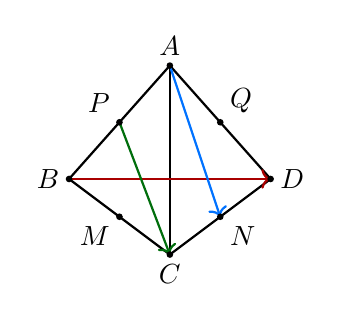
\begin{tikzpicture}[scale=0.8, baseline=(current bounding box.north)]
		\coordinate (A) at (1.6,3);
		\coordinate (B) at (0,1.2);
		\coordinate (C) at (1.6,0);
		\coordinate (D) at (3.2,1.2);
		\coordinate (P) at ($(A)!0.5!(B)$);
		\coordinate (Q) at ($(A)!0.5!(D)$);
		\coordinate (M) at ($(B)!0.5!(C)$);
		\coordinate (N) at ($(C)!0.5!(D)$);
		\draw[thick] (A)--(B)--(C)--(D)--cycle;
		\draw[thick] (A)--(C);
		\draw[thick, dashed] (B)--(D);
		% 化简结果向量
		\draw[->, thick, DarkRed] (B)--(D);   % (1) BD
		\draw[->, thick, SkyBlue] (A)--(N);   % (2) AN
		\draw[->, thick, DarkGreen] (P)--(C); % (3) PC
		\foreach \p/\pos in {A/above, B/left, C/below, D/right}
		\fill (\p) circle (1.5pt) node[\pos] {$\p$};
		\foreach \p/\pos in {P/above left, Q/above right, M/below left, N/below right}
		\fill (\p) circle (1.5pt) node[\pos] {$\p$};
	\end{tikzpicture}
\end{minipage}

\category{过关练习\quad $\bigstar\bigstar$}

\begin{minipage}[t]{0.7\textwidth}
	\begin{question}[2020\textasciitilde2021学年陕西西安新城区西安市第八十九中学高二上学期期中理科]
		如图，在四面体$OABC$中，$D$是$BC$的中点，$G$是$AD$的中点，则$\overrightarrow{OG}$等于（\quad C\quad）
		
		\begin{tabular}{@{}l@{\quad}l@{}}
			A. $\dfrac{1}{3}\overrightarrow{OA}+\dfrac{1}{3}\overrightarrow{OB}+\dfrac{1}{3}\overrightarrow{OC}$ &
			B. $\dfrac{1}{2}\overrightarrow{OA}+\dfrac{1}{3}\overrightarrow{OB}+\dfrac{1}{4}\overrightarrow{OC}$ \\[10pt]
			C. $\dfrac{1}{2}\overrightarrow{OA}+\dfrac{1}{4}\overrightarrow{OB}+\dfrac{1}{4}\overrightarrow{OC}$ &
			D. $\dfrac{1}{4}\overrightarrow{OA}+\dfrac{1}{4}\overrightarrow{OB}+\dfrac{1}{6}\overrightarrow{OC}$
		\end{tabular}
	\end{question}
	解：$\because D$是$BC$中点，$\therefore \overrightarrow{OD}=\dfrac{1}{2}\left(\overrightarrow{OB}+\overrightarrow{OC}\right)$；
	$\because G$是$AD$中点，
	\[
	\overrightarrow{OG}=\frac{1}{2}\left(\overrightarrow{OA}+\overrightarrow{OD}\right)=\frac{1}{2}\overrightarrow{OA}+\frac{1}{4}\overrightarrow{OB}+\frac{1}{4}\overrightarrow{OC}
	\]
	故选 C.
\end{minipage}
\hfill
\begin{minipage}[t]{0.3\textwidth}
	\centering
	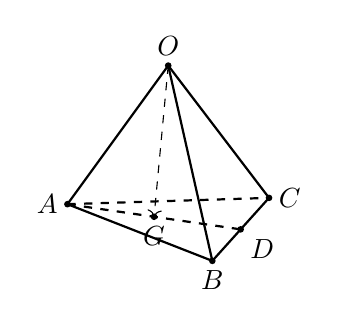
\begin{tikzpicture}[scale=0.8, baseline=(current bounding box.north)]
		\coordinate (O) at (1.6,3.2);
		\coordinate (A) at (0,1);
		\coordinate (B) at (2.3,0.1);
		\coordinate (C) at (3.2,1.1);
		\coordinate (D) at ($(B)!0.5!(C)$);
		\coordinate (G) at ($(A)!0.5!(D)$);
		\draw[thick] (O)--(A); \draw[thick] (O)--(B); \draw[thick] (O)--(C);
		\draw[thick] (A)--(B)--(C);
		\draw[thick, dashed] (A)--(C);
		\draw[thick, dashed] (A)--(D);
		\draw[->, dashed] (O)--(G);
		\foreach \p/\pos in {O/above, A/left, B/below, C/right}
		\fill (\p) circle (1.5pt) node[\pos] {$\p$};
		\fill (D) circle (1.5pt) node[below right] {$D$};
		\fill (G) circle (1.5pt) node[below] {$G$};
	\end{tikzpicture}
\end{minipage}

\category{思维延伸\quad $\bigstar\bigstar\bigstar$}

\begin{minipage}[t]{0.7\textwidth}
	\begin{question}
		在三棱锥$O-ABC$中，点$M$，$N$分别为$OA$，$BC$的中点，若$\overrightarrow{OG}=\dfrac{1}{3}\overrightarrow{OA}+x\overrightarrow{OB}+y\overrightarrow{OC}$，且$G$，$M$，$N$三点共线，则$x+y=$（\quad B\quad）
		
		\begin{tabular}{@{}l@{\quad}l@{\quad}l@{\quad}l@{}}
			A. $-\dfrac{1}{3}$ & B. $\dfrac{1}{3}$ & C. $\dfrac{2}{3}$ & D. $-\dfrac{2}{3}$
		\end{tabular}
	\end{question}
	解：由$G,M,N$共线，设$\overrightarrow{OG}=m\overrightarrow{OM}+(1-m)\overrightarrow{ON}$.
	又$\overrightarrow{OM}=\dfrac{1}{2}\overrightarrow{OA}$，$\overrightarrow{ON}=\dfrac{1}{2}\left(\overrightarrow{OB}+\overrightarrow{OC}\right)$，
	\[
	\overrightarrow{OG}=\frac{m}{2}\overrightarrow{OA}+\frac{1-m}{2}\overrightarrow{OB}+\frac{1-m}{2}\overrightarrow{OC}
	\]
	对照系数：$\dfrac{m}{2}=\dfrac{1}{3}\implies m=\dfrac{2}{3}$，
	\[
	\therefore x=y=\frac{1-m}{2}=\frac{1}{6},\quad x+y=\frac{1}{3}
	\]
	故选 B.
\end{minipage}
\hfill
\begin{minipage}[t]{0.3\textwidth}
	\centering
	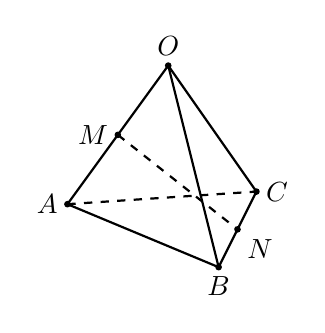
\begin{tikzpicture}[scale=0.8, baseline=(current bounding box.north)]
		\coordinate (O) at (1.6,3.2);
		\coordinate (A) at (0,1);
		\coordinate (B) at (2.4,0);
		\coordinate (C) at (3,1.2);
		\coordinate (M) at ($(O)!0.5!(A)$);
		\coordinate (N) at ($(B)!0.5!(C)$);
		\draw[thick] (O)--(A)--(B)--(C)--(O);
		\draw[thick] (O)--(B);
		\draw[thick, dashed] (A)--(C);
		\draw[thick, dashed] (M)--(N);
		\foreach \p/\pos in {O/above, A/left, B/below, C/right}
		\fill (\p) circle (1.5pt) node[\pos] {$\p$};
		\fill (M) circle (1.5pt) node[left] {$M$};
		\fill (N) circle (1.5pt) node[below right] {$N$};
	\end{tikzpicture}
\end{minipage}

% ================= 教师版（有答案） =================
\category{例题2·(1)\quad $\bigstar\bigstar$}

\begin{minipage}[t]{0.7\textwidth}
	\begin{question}
		已知$\overrightarrow{a}$，$\overrightarrow{b}$，$\overrightarrow{c}$是三个不共面的向量，试判断向量$\overrightarrow{a}+2\overrightarrow{b}$，$2\overrightarrow{b}+3\overrightarrow{c}$，$-9\overrightarrow{c}+3\overrightarrow{a}$是否共面.
	\end{question}
	解：$\because \overrightarrow{a},\overrightarrow{b},\overrightarrow{c}$不共面，$\therefore \overrightarrow{a}+2\overrightarrow{b}$与$2\overrightarrow{b}+3\overrightarrow{c}$不共线.
	
	假设$-9\overrightarrow{c}+3\overrightarrow{a}=x(\overrightarrow{a}+2\overrightarrow{b})+y(2\overrightarrow{b}+3\overrightarrow{c})$，即
	\[
	3\overrightarrow{a}+0\overrightarrow{b}-9\overrightarrow{c}=x\overrightarrow{a}+(2x+2y)\overrightarrow{b}+3y\overrightarrow{c}
	\]
	由$\overrightarrow{a},\overrightarrow{b},\overrightarrow{c}$不共面，对应系数相等：
	\[
	\begin{cases}
		x=3\\
		2x+2y=0\\
		3y=-9
	\end{cases}
	\]
	解得$x=3,\ y=-3$，代入$2x+2y=0$成立.
	\[
	\therefore -9\overrightarrow{c}+3\overrightarrow{a}=3(\overrightarrow{a}+2\overrightarrow{b})-3(2\overrightarrow{b}+3\overrightarrow{c})
	\]
	故向量$\overrightarrow{a}+2\overrightarrow{b}$，$2\overrightarrow{b}+3\overrightarrow{c}$，$-9\overrightarrow{c}+3\overrightarrow{a}$\textbf{共面}.
\end{minipage}
\hfill
\begin{minipage}[t]{0.3\textwidth}
	\centering
	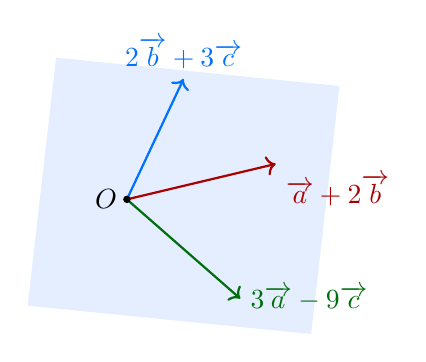
\begin{tikzpicture}[scale=0.9, baseline=(current bounding box.north)]
		% 示意平面
		\fill[LightBlue] (-1.2,-1.5) -- (2.8,-1.9) -- (3.2,1.6) -- (-0.8,2) -- cycle;
		\coordinate (O) at (0.2,0);
		\draw[->, thick, DarkRed] (O) -- (2.3,0.5) node[below right] {$\overrightarrow{a}+2\overrightarrow{b}$};
		\draw[->, thick, SkyBlue] (O) -- (1,1.7) node[above] {$2\overrightarrow{b}+3\overrightarrow{c}$};
		\draw[->, thick, DarkGreen] (O) -- (1.8,-1.4) node[right] {$3\overrightarrow{a}-9\overrightarrow{c}$};
		\fill (O) circle (1.5pt) node[left] {$O$};
	\end{tikzpicture}
\end{minipage}

\category{例题2·(2)\quad $\bigstar\bigstar$}

\begin{minipage}[t]{0.7\textwidth}
	\begin{question}
		设空间中的任意一点$O$和不共线的三点$A$、$B$、$C$，若$P$点满足关系$\overrightarrow{OP}=x\overrightarrow{OA}+y\overrightarrow{OB}+z\overrightarrow{OC}$，且$x+y+z=1$，证明：$A$、$B$、$C$、$P$四点共面.
	\end{question}
	证明：$\because x+y+z=1$，$\therefore x=1-y-z$，
	\[
	\overrightarrow{OP}=(1-y-z)\overrightarrow{OA}+y\overrightarrow{OB}+z\overrightarrow{OC}
	\]
	\[
	\overrightarrow{OP}-\overrightarrow{OA}=y(\overrightarrow{OB}-\overrightarrow{OA})+z(\overrightarrow{OC}-\overrightarrow{OA})
	\]
	即
	\[
	\overrightarrow{AP}=y\overrightarrow{AB}+z\overrightarrow{AC}
	\]
	$\because A$、$B$、$C$不共线，由共面向量定理，$\overrightarrow{AP}$与$\overrightarrow{AB},\overrightarrow{AC}$共面，
	又它们有公共点$A$，
	$\therefore A$、$B$、$C$、$P$四点共面. $\blacksquare$
\end{minipage}
\hfill
\begin{minipage}[t]{0.3\textwidth}
	\centering
	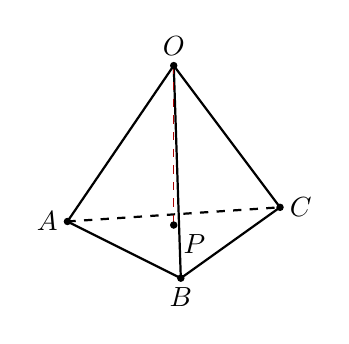
\begin{tikzpicture}[scale=0.9, baseline=(current bounding box.north)]
		\coordinate (O) at (1.5,3);
		\coordinate (A) at (0,0.8);
		\coordinate (B) at (1.6,0);
		\coordinate (C) at (3,1);
		\coordinate (P) at (1.5,0.75);
		\draw[thick] (O)--(A); \draw[thick] (O)--(B); \draw[thick] (O)--(C);
		\draw[thick] (A)--(B)--(C);
		\draw[thick, dashed] (A)--(C);
		\draw[dashed, DarkRed] (O)--(P);
		\foreach \p/\pos in {O/above, A/left, B/below, C/right}
		\fill (\p) circle (1.5pt) node[\pos] {$\p$};
		\fill (P) circle (1.5pt) node[below right] {$P$};
	\end{tikzpicture}
\end{minipage}

% ================= 教师版（有答案） =================
\category{过关练习·1\quad $\bigstar\bigstar$}

\begin{question}
	已知$\overrightarrow{a}$，$\overrightarrow{b}$，$\overrightarrow{c}$是三个不共面的向量，若$\overrightarrow{p}=2\overrightarrow{a}-\overrightarrow{b}+2\overrightarrow{c}$，$\overrightarrow{q}=-\overrightarrow{a}+3\overrightarrow{b}-3\overrightarrow{c}$，$\overrightarrow{r}=13\overrightarrow{a}+6\overrightarrow{b}+\lambda\overrightarrow{c}$，若向量$\overrightarrow{p}$，$\overrightarrow{q}$，$\overrightarrow{r}$共面，则$\lambda=$（\quad B\quad）
	
	\begin{tabular}{@{}l@{\quad}l@{\quad}l@{\quad}l@{}}
		A. $2$ & B. $3$ & C. $4$ & D. $6$
	\end{tabular}
\end{question}
解：由三向量共面，设$\overrightarrow{r}=x\overrightarrow{p}+y\overrightarrow{q}$，即
\[
13\overrightarrow{a}+6\overrightarrow{b}+\lambda\overrightarrow{c}=x(2\overrightarrow{a}-\overrightarrow{b}+2\overrightarrow{c})+y(-\overrightarrow{a}+3\overrightarrow{b}-3\overrightarrow{c})
\]
\[
13\overrightarrow{a}+6\overrightarrow{b}+\lambda\overrightarrow{c}=(2x-y)\overrightarrow{a}+(-x+3y)\overrightarrow{b}+(2x-3y)\overrightarrow{c}
\]
由$\overrightarrow{a},\overrightarrow{b},\overrightarrow{c}$不共面，对应系数相等：
\[
\begin{cases}
	2x-y=13\\
	-x+3y=6\\
	\lambda=2x-3y
\end{cases}
\]
解得$x=9,\ y=5$，代入得$\lambda=2\times9-3\times5=3$，故选 B.

\category{过关练习·2\quad $\bigstar\bigstar\bigstar$}

\begin{question}
	已知$O$为空间任意一点，$A$，$B$，$C$，$P$满足任意三点不共线，但四点共面，且$\overrightarrow{BP}=m\overrightarrow{OA}+\overrightarrow{OB}+\overrightarrow{OC}$，则$m$的值为（\quad C\quad）
	
	\begin{tabular}{@{}l@{\quad}l@{\quad}l@{\quad}l@{}}
		A. $-1$ & B. $2$ & C. $-2$ & D. $-3$
	\end{tabular}
\end{question}
解：$\overrightarrow{OP}=\overrightarrow{OB}+\overrightarrow{BP}=m\overrightarrow{OA}+2\overrightarrow{OB}+\overrightarrow{OC}$.

四点共面且起点相同，则系数之和为$1$：
\[
m+2+1=1 \implies m=-2
\]
故选 C.

\subsection{向量的数量积}
\begin{knowledge}{数量积}
	已知两个非零向量$\overrightarrow{a}$，$\overrightarrow{b}$，在空间任取一点$O$，作$\overrightarrow{OA}=\overrightarrow{a}$，$\overrightarrow{OB}=\overrightarrow{b}$，则$\angle AOB$叫做向量$\overrightarrow{a}$，$\overrightarrow{b}$的夹角，记作$\langle\overrightarrow{a},\overrightarrow{b}\rangle$.
	
	已知两个非零向量$\overrightarrow{a}$，$\overrightarrow{b}$，则$|\overrightarrow{a}||\overrightarrow{b}|\cos\langle\overrightarrow{a},\overrightarrow{b}\rangle$叫做$\overrightarrow{a}$，$\overrightarrow{b}$的数量积，记作
	\[
	\overrightarrow{a}\cdot\overrightarrow{b}=|\overrightarrow{a}||\overrightarrow{b}|\cos\langle\overrightarrow{a},\overrightarrow{b}\rangle
	\]
\end{knowledge}

\begin{knowledge}{空间向量的数量积运算律}
	\begin{enumerate}[label=(\arabic*)]
		\item 与实数的结合律：$(\lambda\overrightarrow{a})\cdot\overrightarrow{b}=\lambda(\overrightarrow{a}\cdot\overrightarrow{b})$
		\item 交换律：$\overrightarrow{a}\cdot\overrightarrow{b}=\overrightarrow{b}\cdot\overrightarrow{a}$
		\item 分配律：$\overrightarrow{a}\cdot(\overrightarrow{b}+\overrightarrow{c})=\overrightarrow{a}\cdot\overrightarrow{b}+\overrightarrow{a}\cdot\overrightarrow{c}$
	\end{enumerate}
	
	\begin{minipage}[t]{0.7\textwidth}
		$\overrightarrow{b}$在$\overrightarrow{a}$上的投影：
		\[
		|\overrightarrow{b}|\cdot\cos\langle\overrightarrow{a},\overrightarrow{b}\rangle
		\]
		
		$\overrightarrow{b}$在$\overrightarrow{a}$上的投影向量：
		\[
		|\overrightarrow{b}|\cdot\cos\langle\overrightarrow{a},\overrightarrow{b}\rangle\cdot\frac{\overrightarrow{a}}{|\overrightarrow{a}|}
		\]
		
		\textbf{注意：}投影是数量，锐角时为正、钝角时为负、直角时为$0$；投影向量是向量，方向与$\overrightarrow{a}$相同（图中$\theta=\langle\overrightarrow{a},\overrightarrow{b}\rangle$）.
	\end{minipage}
	\hfill
	\begin{minipage}[t]{0.3\textwidth}
		\centering
		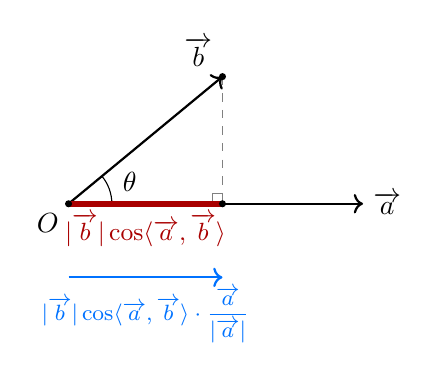
\begin{tikzpicture}[scale=0.85, baseline=(current bounding box.north)]
			\coordinate (O) at (0,0);
			\coordinate (A) at (4.4,0);
			\coordinate (B) at (2.3,1.9);
			\coordinate (H) at (2.3,0);
			% 向量 a、b
			\draw[->, thick] (O) -- (A) node[right] {$\overrightarrow{a}$};
			\draw[->, thick] (O) -- (B) node[above left] {$\overrightarrow{b}$};
			% 垂线与直角标记
			\draw[dashed, gray] (B) -- (H);
			\draw[gray] (H) ++(-0.15,0) -- ++(0,0.15) -- ++(0.15,0);
			% 夹角
			\draw pic["$\theta$", draw, angle eccentricity=1.5, angle radius=0.55cm] {angle = A--O--B};
			% 投影（数量，红色粗线段 OH）
			\draw[DarkRed, line width=2pt] (O) -- (H);
			\node[below, DarkRed] at (1.15,0) {\small$|\overrightarrow{b}|\cos\langle\overrightarrow{a},\overrightarrow{b}\rangle$};
			% 投影向量（蓝色箭头，方向与 a 相同）
			\draw[->, thick, SkyBlue] (0,-1.1) -- (2.3,-1.1);
			\node[below, SkyBlue] at (1.15,-1.1) {\footnotesize$|\overrightarrow{b}|\cos\langle\overrightarrow{a},\overrightarrow{b}\rangle\cdot\dfrac{\overrightarrow{a}}{|\overrightarrow{a}|}$};
			% 标点
			\fill (O) circle (1.5pt) node[below left] {$O$};
			\fill (B) circle (1.5pt);
			\fill (H) circle (1.5pt);
		\end{tikzpicture}
	\end{minipage}
\end{knowledge}

% ================= 教师版（有答案） =================
\category{例题3\quad $\bigstar\bigstar\bigstar$}

\begin{minipage}[t]{0.7\textwidth}
	\begin{question}[2020\textasciitilde2021学年湖北武汉洪山区华中师范大学第一附属中学高二上学期期中第10题]
		（多选）在平行六面体$ABCD-A_1B_1C_1D_1$中，$\angle BAD=\angle A_1AB=\angle A_1AD=\dfrac{\pi}{3}$，各棱长均为$1$，则下列命题中正确的是（\quad ACD\quad）
		
		\begin{tabular}{@{}l@{}}
			A. $\left\{\overrightarrow{AC},\overrightarrow{AC_1},\overrightarrow{BB_1}\right\}$不是空间的一个基底 \\[6pt]
			B. $\langle\overrightarrow{AD},\overrightarrow{DD_1}\rangle=\dfrac{2}{3}\pi$ \\[6pt]
			C. $|\overrightarrow{BD_1}|=\sqrt{2}$ \\[6pt]
			D. $BD\perp$平面$ACC_1A_1$
		\end{tabular}
	\end{question}
	解：设$\overrightarrow{AB}=\overrightarrow{a}$，$\overrightarrow{AD}=\overrightarrow{b}$，$\overrightarrow{AA_1}=\overrightarrow{c}$，则$|\overrightarrow{a}|=|\overrightarrow{b}|=|\overrightarrow{c}|=1$，$\overrightarrow{a}\cdot\overrightarrow{b}=\overrightarrow{b}\cdot\overrightarrow{c}=\overrightarrow{c}\cdot\overrightarrow{a}=\dfrac{1}{2}$.
	\begin{enumerate}[label=\Alph*.]
		\item $\overrightarrow{AC_1}-\overrightarrow{AC}=\overrightarrow{CC_1}=\overrightarrow{BB_1}$，三向量共面，不能构成基底，正确；
		\item $\langle\overrightarrow{AD},\overrightarrow{DD_1}\rangle=\langle\overrightarrow{b},\overrightarrow{c}\rangle=\dfrac{\pi}{3}$，错误；
		\item $\overrightarrow{BD_1}=\overrightarrow{b}+\overrightarrow{c}-\overrightarrow{a}$，
		$|\overrightarrow{BD_1}|^2=1+1+1+2\cdot\dfrac{1}{2}-2\cdot\dfrac{1}{2}-2\cdot\dfrac{1}{2}=2$，即$|\overrightarrow{BD_1}|=\sqrt{2}$，正确；
		\item $\overrightarrow{BD}=\overrightarrow{b}-\overrightarrow{a}$，$\overrightarrow{BD}\cdot\overrightarrow{AC}=(\overrightarrow{b}-\overrightarrow{a})\cdot(\overrightarrow{a}+\overrightarrow{b})=|\overrightarrow{b}|^2-|\overrightarrow{a}|^2=0$，
		$\overrightarrow{BD}\cdot\overrightarrow{AA_1}=(\overrightarrow{b}-\overrightarrow{a})\cdot\overrightarrow{c}=0$，
		$\therefore BD\perp AC$，$BD\perp AA_1$，又$AC\cap AA_1=A$，$\therefore BD\perp$平面$ACC_1A_1$，正确.
	\end{enumerate}
	故选 ACD.
\end{minipage}
\hfill
\begin{minipage}[t]{0.3\textwidth}
	\centering
	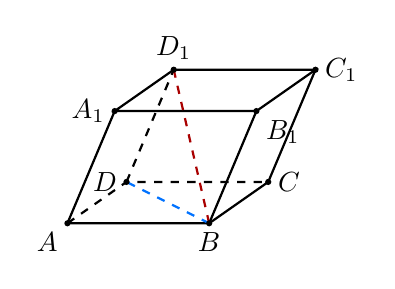
\begin{tikzpicture}[scale=0.75, baseline=(current bounding box.north)]
		\coordinate (A) at (0,0);
		\coordinate (B) at (2.4,0);
		\coordinate (C) at (3.4,0.7);
		\coordinate (D) at (1,0.7);
		\coordinate (A1) at (0.8,1.9);
		\coordinate (B1) at (3.2,1.9);
		\coordinate (C1) at (4.2,2.6);
		\coordinate (D1) at (1.8,2.6);
		\draw[thick] (A)--(B)--(C);
		\draw[thick, dashed] (A)--(D)--(C);
		\draw[thick] (A1)--(B1)--(C1)--(D1)--cycle;
		\draw[thick] (A)--(A1);
		\draw[thick] (B)--(B1);
		\draw[thick] (C)--(C1);
		\draw[thick, dashed] (D)--(D1);
		\draw[thick, dashed, SkyBlue] (B)--(D);
		\draw[thick, dashed, DarkRed] (B)--(D1);
		\fill (A) circle (1.5pt) node[below left] {$A$};
		\fill (B) circle (1.5pt) node[below] {$B$};
		\fill (C) circle (1.5pt) node[right] {$C$};
		\fill (D) circle (1.5pt) node[left] {$D$};
		\fill (A1) circle (1.5pt) node[left] {$A_1$};
		\fill (B1) circle (1.5pt) node[below right] {$B_1$};
		\fill (C1) circle (1.5pt) node[right] {$C_1$};
		\fill (D1) circle (1.5pt) node[above] {$D_1$};
	\end{tikzpicture}
\end{minipage}

\category{过关练习\quad $\bigstar\bigstar$}

\begin{minipage}[t]{0.7\textwidth}
	\begin{question}[2020\textasciitilde2021学年天津滨海新区塘沽第一中学高二上学期期中第8题]
		如图，平行六面体$ABCD-A'B'C'D'$，其中$AB=4$，$AD=3$，$AA'=3$，$\angle BAD=90^\circ$，$\angle BAA'=60^\circ$，$\angle DAA'=60^\circ$，则$AC'$的长为（\quad A\quad）
		
		\begin{tabular}{@{}l@{\quad}l@{\quad}l@{\quad}l@{}}
			A. $\sqrt{55}$ & B. $\sqrt{65}$ & C. $\sqrt{85}$ & D. $\sqrt{95}$
		\end{tabular}
	\end{question}
	解：$\overrightarrow{AC'}=\overrightarrow{AB}+\overrightarrow{AD}+\overrightarrow{AA'}$，
	其中$\overrightarrow{AB}\cdot\overrightarrow{AD}=0$，$\overrightarrow{AB}\cdot\overrightarrow{AA'}=4\times3\times\dfrac{1}{2}=6$，$\overrightarrow{AD}\cdot\overrightarrow{AA'}=3\times3\times\dfrac{1}{2}=\dfrac{9}{2}$.
	\[
	|\overrightarrow{AC'}|^2=16+9+9+2\left(0+6+\frac{9}{2}\right)=34+21=55
	\]
	$\therefore |AC'|=\sqrt{55}$，故选 A.
\end{minipage}
\hfill
\begin{minipage}[t]{0.3\textwidth}
	\centering
	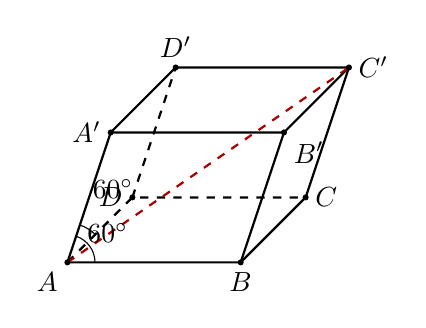
\begin{tikzpicture}[scale=0.55, baseline=(current bounding box.north)]
		\coordinate (A) at (0,0);
		\coordinate (B) at (4,0);
		\coordinate (C) at (5.5,1.5);
		\coordinate (D) at (1.5,1.5);
		\coordinate (A') at (1,3);
		\coordinate (B') at (5,3);
		\coordinate (C') at (6.5,4.5);
		\coordinate (D') at (2.5,4.5);
		\draw[thick] (A)--(B)--(C);
		\draw[thick, dashed] (A)--(D)--(C);
		\draw[thick] (A')--(B')--(C')--(D')--cycle;
		\draw[thick] (A)--(A');
		\draw[thick] (B)--(B');
		\draw[thick] (C)--(C');
		\draw[thick, dashed] (D)--(D');
		\draw[thick, dashed, DarkRed] (A)--(C');
		\fill (A) circle (2pt) node[below left] {$A$};
		\fill (B) circle (2pt) node[below] {$B$};
		\fill (C) circle (2pt) node[right] {$C$};
		\fill (D) circle (2pt) node[left] {$D$};
		\fill (A') circle (2pt) node[left] {$A'$};
		\fill (B') circle (2pt) node[below right] {$B'$};
		\fill (C') circle (2pt) node[right] {$C'$};
		\fill (D') circle (2pt) node[above] {$D'$};
		\draw pic["$60^\circ$", draw, angle eccentricity=1.8, angle radius=0.35cm] {angle = B--A--A'};
		\draw pic["$60^\circ$", draw, angle eccentricity=2.2, angle radius=0.5cm] {angle = D--A--A'};
	\end{tikzpicture}
\end{minipage}

\subsection{空间向量的坐标运算}
\begin{minipage}[t]{0.7\textwidth}
	\begin{knowledge}{空间直角坐标系}
		在空间选定一点$O$和一个单位正交基底$\left\{\overrightarrow{i},\overrightarrow{j},\overrightarrow{k}\right\}$，以点$O$为原点，分别以$\overrightarrow{i},\overrightarrow{j},\overrightarrow{k}$的方向为正方向、以它们的长为单位长度建立三条数轴：$x$轴、$y$轴、$z$轴，它们都叫做坐标轴.这时我们就建立了一个空间直角坐标系$Oxyz$，$O$叫做原点，$\overrightarrow{i},\overrightarrow{j},\overrightarrow{k}$都叫做坐标向量，通过每两条坐标轴的平面叫做坐标平面.
		
		对于空间任一向量$\overrightarrow{a}$，存在一组有序实数$(x,y,z)$，使得$\overrightarrow{a}=x\overrightarrow{i}+y\overrightarrow{j}+z\overrightarrow{k}$，我们把$\overrightarrow{a}=x\overrightarrow{i}+y\overrightarrow{j}+z\overrightarrow{k}$叫做向量$\overrightarrow{a}$的标准正交分解，把$\overrightarrow{i},\overrightarrow{j},\overrightarrow{k}$叫做\textbf{标准正交基底}.
	\end{knowledge}
\end{minipage}
\hfill
\begin{minipage}[t]{0.3\textwidth}
	\centering
	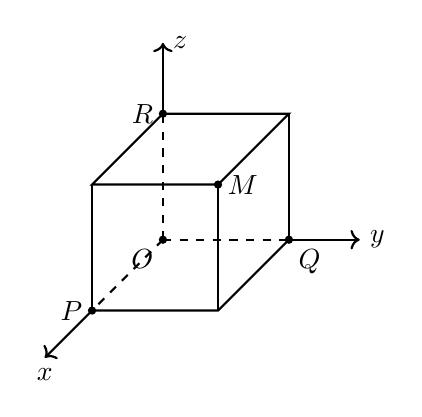
\begin{tikzpicture}[scale=1, baseline=(current bounding box.north)]
		\coordinate (O) at (0,0);
		\coordinate (P) at (-0.9,-0.9);
		\coordinate (Q) at (1.6,0);
		\coordinate (R) at (0,1.6);
		\coordinate (PQ) at (0.7,-0.9);
		\coordinate (PR) at (-0.9,0.7);
		\coordinate (QR) at (1.6,1.6);
		\coordinate (M) at (0.7,0.7);
		% 隐藏棱（坐标轴在体内部分）
		\draw[thick, dashed] (O)--(P);
		\draw[thick, dashed] (O)--(Q);
		\draw[thick, dashed] (O)--(R);
		% 可见棱
		\draw[thick] (P)--(PQ)--(Q);
		\draw[thick] (P)--(PR);
		\draw[thick] (PQ)--(M);
		\draw[thick] (Q)--(QR);
		\draw[thick] (R)--(PR)--(M)--(QR)--(R);
		% 坐标轴
		\draw[->, thick] (P)--(-1.5,-1.5) node[below] {$x$};
		\draw[->, thick] (Q)--(2.5,0) node[right] {$y$};
		\draw[->, thick] (R)--(0,2.5) node[right] {$z$};
		% 标点
		\fill (O) circle (1.5pt) node[below left] {$O$};
		\fill (P) circle (1.5pt) node[left] {$P$};
		\fill (Q) circle (1.5pt) node[below right] {$Q$};
		\fill (R) circle (1.5pt) node[left] {$R$};
		\fill (M) circle (1.5pt) node[right] {$M$};
	\end{tikzpicture}
\end{minipage}

\begin{knowledge}{空间向量运算的坐标表示}
	设$\overrightarrow{a}=(x_1,y_1,z_1)$，$\overrightarrow{b}=(x_2,y_2,z_2)$.
	\begin{itemize}
		\item 向量的加减：$\overrightarrow{a}\pm\overrightarrow{b}=(x_1\pm x_2,\ y_1\pm y_2,\ z_1\pm z_2)$
		\item 数乘向量：$\lambda\overrightarrow{a}=\lambda(x_1,y_1,z_1)=(\lambda x_1,\ \lambda y_1,\ \lambda z_1)$
		\item 数量积：$\overrightarrow{a}\cdot\overrightarrow{b}=x_1x_2+y_1y_2+z_1z_2$
		\item 向量的模：$|\overrightarrow{a}|=\sqrt{x_1^2+y_1^2+z_1^2}$
		\item 向量的夹角：$\cos\langle\overrightarrow{a},\overrightarrow{b}\rangle=\dfrac{x_1x_2+y_1y_2+z_1z_2}{\sqrt{x_1^2+y_1^2+z_1^2}\sqrt{x_2^2+y_2^2+z_2^2}}$
		\item 向量共线：若$\overrightarrow{b}\neq\overrightarrow{0}$，则$\overrightarrow{a}\parallel\overrightarrow{b}\iff\overrightarrow{a}=\lambda\overrightarrow{b}\iff x_1=\lambda x_2,\ y_1=\lambda y_2,\ z_1=\lambda z_2$
		\item 向量垂直：$\overrightarrow{a}\perp\overrightarrow{b}\iff\overrightarrow{a}\cdot\overrightarrow{b}=x_1x_2+y_1y_2+z_1z_2=0$
	\end{itemize}
\end{knowledge}

% ================= 教师版（有答案） =================
\category{例题4·1\quad $\bigstar$}

\begin{question}
	已知$\overrightarrow{a}=(1,2,3)$，$\overrightarrow{b}=(-2,-1,2)$，计算：
\end{question}
解：$|\overrightarrow{a}|=\sqrt{14}$，$|\overrightarrow{b}|=3$.
\begin{enumerate}[label=(\arabic*)]
	\item $\overrightarrow{a}+2\overrightarrow{b}=(1-4,\ 2-2,\ 3+4)=\underline{\ (-3,0,7)\ }$
	\item $\overrightarrow{a}\cdot\overrightarrow{b}=-2-2+6=\underline{\ 2\ }$
	\item $\cos\langle\overrightarrow{a},\overrightarrow{b}\rangle=\dfrac{2}{3\sqrt{14}}=\underline{\ \dfrac{\sqrt{14}}{21}\ }$
	\item $\overrightarrow{a}-\overrightarrow{b}=(3,3,1)$，$|\overrightarrow{a}-\overrightarrow{b}|=\underline{\ \sqrt{19}\ }$
	\item $\overrightarrow{c}\parallel\overrightarrow{a}\implies\overrightarrow{c}=-2\overrightarrow{a}$，$x=\underline{\ -4\ }$，$y=\underline{\ -6\ }$
	\item $\overrightarrow{a}\cdot\overrightarrow{c}=1+4+3m=0\implies m=\underline{\ -\dfrac{5}{3}\ }$
\end{enumerate}

\category{例题4·2\quad $\bigstar\bigstar$}

\begin{question}
	若$A(m+1,n+1,3)$，$B(2m,n,m-2n)$，$C(m+3,n-3,9)$三点共线，则$m+n=\underline{\quad 0\quad}$
\end{question}
解：$\overrightarrow{AB}=(m-1,-1,m-2n-3)$，$\overrightarrow{AC}=(2,-4,6)$.

三点共线：$\overrightarrow{AB}=\lambda\overrightarrow{AC}$，由$y$分量知$\lambda=\dfrac{1}{4}$.
\[
m-1=\frac{2}{4}\implies m=\frac{3}{2},\qquad m-2n-3=\frac{6}{4}\implies n=-\frac{3}{2}
\]
$\therefore m+n=0$.

\category{过关练习\quad $\bigstar$}

\begin{question}[2020\textasciitilde2021学年山东济宁泗水县高二上学期期中第5题]
	已知$A(2,-5,1)$，$B(2,-2,4)$，$C(1,-4,1)$，则向量$\overrightarrow{AB}$与$\overrightarrow{AC}$的夹角为（\quad C\quad）
	
	\begin{tabular}{@{}l@{\quad}l@{\quad}l@{\quad}l@{}}
		A. $30^\circ$ & B. $45^\circ$ & C. $60^\circ$ & D. $90^\circ$
	\end{tabular}
\end{question}
解：$\overrightarrow{AB}=(0,3,3)$，$\overrightarrow{AC}=(-1,1,0)$.
\[
\cos\theta=\frac{\overrightarrow{AB}\cdot\overrightarrow{AC}}{|\overrightarrow{AB}||\overrightarrow{AC}|}=\frac{3}{\sqrt{18}\cdot\sqrt{2}}=\frac{3}{6}=\frac{1}{2}
\]
$\therefore \theta=60^\circ$，故选 C.

% ================= 教师版（有答案） =================
\category{过关练习·2\quad $\bigstar$}

\begin{question}[2019\textasciitilde2020学年江苏南通启东市启东中学高二上学期期中第6题]
	已知两个向量$\overrightarrow{a}=(2,-1,3)$，$\overrightarrow{b}=(4,m,n)$，且$\overrightarrow{a}\parallel\overrightarrow{b}$，则$m+n$的值为（\quad C\quad）
	
	\begin{tabular}{@{}l@{\quad}l@{\quad}l@{\quad}l@{}}
		A. $1$ & B. $2$ & C. $4$ & D. $8$
	\end{tabular}
\end{question}
解：$\overrightarrow{a}\parallel\overrightarrow{b}\implies\overrightarrow{b}=2\overrightarrow{a}$，
$\therefore m=-2,\ n=6$，$m+n=4$，故选 C.

\category{过关练习·3\quad $\bigstar$}

\begin{question}[2021\textasciitilde2022学年广东深圳盐田区深圳外国语学校高二上学期期中第2题]
	已知向量$\overrightarrow{a}=(-2,1,3)$，$\overrightarrow{b}=(-1,2,1)$，若$\overrightarrow{a}\perp(\overrightarrow{a}-\lambda\overrightarrow{b})$，则实数$\lambda$的值为（\quad B\quad）
	
	\begin{tabular}{@{}l@{\quad}l@{\quad}l@{\quad}l@{}}
		A. $-2$ & B. $2$ & C. $\dfrac{14}{5}$ & D. $-\dfrac{14}{3}$
	\end{tabular}
\end{question}
解：$\overrightarrow{a}\cdot(\overrightarrow{a}-\lambda\overrightarrow{b})=|\overrightarrow{a}|^2-\lambda\overrightarrow{a}\cdot\overrightarrow{b}=14-7\lambda=0\implies\lambda=2$，故选 B.

\category{思维延伸·1\quad $\bigstar\bigstar\bigstar$}

\begin{question}[2021\textasciitilde2022学年广东深圳盐田区深圳外国语学校高二上学期期中第6题]
	已知$\overrightarrow{a}=(2,3,-2)$，$\overrightarrow{b}=(-4,2,1)$，$\overrightarrow{c}=(10,3,\lambda)$，若$\overrightarrow{a}$、$\overrightarrow{b}$、$\overrightarrow{c}$三个向量共面，则实数$\lambda$等于（\quad A\quad）
	
	\begin{tabular}{@{}l@{\quad}l@{\quad}l@{\quad}l@{}}
		A. $-\dfrac{11}{2}$ & B. $\dfrac{5}{2}$ & C. $\dfrac{9}{2}$ & D. $\dfrac{7}{2}$
	\end{tabular}
\end{question}
解：三向量共面，设$\overrightarrow{c}=x\overrightarrow{a}+y\overrightarrow{b}$：
\[
\begin{cases}
	2x-4y=10\\
	3x+2y=3\\
	-2x+y=\lambda
\end{cases}
\]
解得$x=2,\ y=-\dfrac{3}{2}$，代入得$\lambda=-4-\dfrac{3}{2}=-\dfrac{11}{2}$，故选 A.

\category{思维延伸·2\quad $\bigstar\bigstar\bigstar$}

\begin{question}
	从点$A(2,-1,7)$沿向量$\overrightarrow{a}=(8,9,-12)$的方向取线段长$|AB|=34$，则$B$点的坐标为（\quad A\quad）
	
	\begin{tabular}{@{}l@{\quad}l@{\quad}l@{\quad}l@{}}
		A. $(18,17,-17)$ & B. $(-14,-19,17)$ & C. $\left(6,\dfrac{7}{2},1\right)$ & D. $\left(-2,-\dfrac{11}{2},13\right)$
	\end{tabular}
\end{question}
解：$\overrightarrow{AB}=\lambda\overrightarrow{a}\ (\lambda>0)$，$|\overrightarrow{a}|=\sqrt{8^2+9^2+12^2}=\sqrt{289}=17$.
\[
|AB|=17\lambda=34\implies\lambda=2
\]
$\therefore B=(2+16,\ -1+18,\ 7-24)=(18,17,-17)$，故选 A.

% ================= 教师版（有答案） =================
\subsection{加油站}
\category{1\quad $\bigstar\bigstar$}

\begin{minipage}[t]{0.7\textwidth}
	\begin{question}
		直三棱柱$ABC-A_1B_1C_1$中，若$\overrightarrow{CA}=\overrightarrow{a}$，$\overrightarrow{CB}=\overrightarrow{b}$，$\overrightarrow{CC_1}=\overrightarrow{c}$，则$\overrightarrow{A_1B}=\underline{\quad-\overrightarrow{a}+\overrightarrow{b}-\overrightarrow{c}\quad}$
	\end{question}
	解：$\overrightarrow{A_1B}=\overrightarrow{A_1A}+\overrightarrow{AB}=-\overrightarrow{c}+(\overrightarrow{b}-\overrightarrow{a})=-\overrightarrow{a}+\overrightarrow{b}-\overrightarrow{c}$.
\end{minipage}
\hfill
\begin{minipage}[t]{0.3\textwidth}
	\centering
	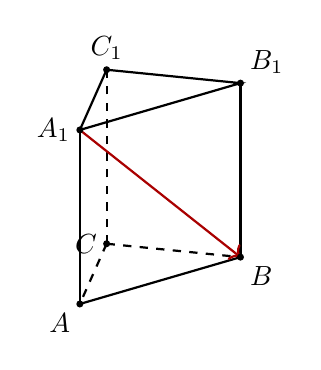
\begin{tikzpicture}[scale=0.85, baseline=(current bounding box.north)]
		\coordinate (A) at (0.8,0);
		\coordinate (B) at (3.2,0.7);
		\coordinate (C) at (1.2,0.9);
		\coordinate (A1) at (0.8,2.6);
		\coordinate (B1) at (3.2,3.3);
		\coordinate (C1) at (1.2,3.5);
		\draw[thick] (A)--(B);
		\draw[thick, dashed] (C)--(A);
		\draw[thick, dashed] (C)--(B);
		\draw[thick] (A)--(A1);
		\draw[thick] (B)--(B1);
		\draw[thick, dashed] (C)--(C1);
		\draw[thick] (A1)--(B1)--(C1)--cycle;
		\draw[->, thick, DarkRed] (A1)--(B);
		\fill (A) circle (1.5pt) node[below left] {$A$};
		\fill (B) circle (1.5pt) node[below right] {$B$};
		\fill (C) circle (1.5pt) node[left] {$C$};
		\fill (A1) circle (1.5pt) node[left] {$A_1$};
		\fill (B1) circle (1.5pt) node[above right] {$B_1$};
		\fill (C1) circle (1.5pt) node[above] {$C_1$};
	\end{tikzpicture}
\end{minipage}

\category{2\quad $\bigstar\bigstar$}

\begin{question}
	已知在空间四边形$ABCD$中，$\overrightarrow{AB}=\overrightarrow{a}$，$\overrightarrow{BC}=\overrightarrow{b}$，$\overrightarrow{AD}=\overrightarrow{c}$，则$\overrightarrow{CD}=\underline{\quad-\overrightarrow{a}-\overrightarrow{b}+\overrightarrow{c}\quad}$
\end{question}
解：$\overrightarrow{CD}=\overrightarrow{AD}-\overrightarrow{AC}=\overrightarrow{c}-(\overrightarrow{a}+\overrightarrow{b})=-\overrightarrow{a}-\overrightarrow{b}+\overrightarrow{c}$.

\category{3\quad $\bigstar\bigstar$}

\begin{minipage}[t]{0.7\textwidth}
	\begin{question}
		空间四边形$ABCD$中，若向量$\overrightarrow{AB}=(-3,5,2)$，$\overrightarrow{CD}=(-7,-1,-4)$，点$E$，$F$分别为线段$BC$，$AD$的中点，则$\overrightarrow{EF}=\underline{\quad(-2,-3,-3)\quad}$
	\end{question}
	解：$\because E,F$分别为$BC,AD$中点，
	\[
	\overrightarrow{EF}=\frac{1}{2}(\overrightarrow{BA}+\overrightarrow{CD})=\frac{1}{2}[(3,-5,-2)+(-7,-1,-4)]=\frac{1}{2}(-4,-6,-6)=(-2,-3,-3)
	\]
\end{minipage}
\hfill
\begin{minipage}[t]{0.3\textwidth}
	\centering
	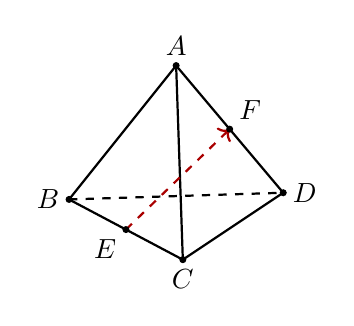
\begin{tikzpicture}[scale=0.85, baseline=(current bounding box.north)]
		\coordinate (A) at (1.6,3);
		\coordinate (B) at (0,1);
		\coordinate (C) at (1.7,0.1);
		\coordinate (D) at (3.2,1.1);
		\coordinate (E) at ($(B)!0.5!(C)$);
		\coordinate (F) at ($(A)!0.5!(D)$);
		\draw[thick] (A)--(B);
		\draw[thick] (B)--(C);
		\draw[thick] (C)--(D);
		\draw[thick] (D)--(A);
		\draw[thick] (A)--(C);
		\draw[thick, dashed] (B)--(D);
		\draw[->, thick, dashed, DarkRed] (E)--(F);
		\fill (A) circle (1.5pt) node[above] {$A$};
		\fill (B) circle (1.5pt) node[left] {$B$};
		\fill (C) circle (1.5pt) node[below] {$C$};
		\fill (D) circle (1.5pt) node[right] {$D$};
		\fill (E) circle (1.5pt) node[below left] {$E$};
		\fill (F) circle (1.5pt) node[above right] {$F$};
	\end{tikzpicture}
\end{minipage}

\category{4\quad $\bigstar\bigstar$}

\begin{question}
	已知$A,B,C$三点不共线，点$O$为平面$ABC$外的一点，则下列条件中，能得到$P\in$平面$ABC$的是（\quad B\quad）
	
	\begin{tabular}{@{}l@{\quad}l@{}}
		A. $\overrightarrow{OP}=\dfrac{1}{3}\overrightarrow{OA}-\dfrac{2}{3}\overrightarrow{OB}+\dfrac{1}{3}\overrightarrow{OC}$ &
		B. $\overrightarrow{OP}=\dfrac{2}{3}\overrightarrow{OA}+\dfrac{4}{3}\overrightarrow{OB}-\overrightarrow{OC}$ \\[12pt]
		C. $\overrightarrow{OP}=\overrightarrow{OA}+\overrightarrow{OB}+\overrightarrow{OC}$ &
		D. $\overrightarrow{OP}=\overrightarrow{OA}-\overrightarrow{OB}-\overrightarrow{OC}$
	\end{tabular}
\end{question}
解：四点共面且起点相同，则系数之和为$1$.
A. $\dfrac{1}{3}-\dfrac{2}{3}+\dfrac{1}{3}=0$；B. $\dfrac{2}{3}+\dfrac{4}{3}-1=1$；C. $3$；D. $-1$.
故选 B.

% ================= 教师版（有答案） =================
\category{5\quad $\bigstar\bigstar$}

\begin{question}
	在四面体$O-ABC$中，已知点$M$在线段$OA$上，且$OM=2MA$，$N$为$BC$的中点，若$\overrightarrow{OG}=\dfrac{1}{3}\overrightarrow{OA}+\dfrac{x}{4}\overrightarrow{OB}+\dfrac{x}{4}\overrightarrow{OC}$，则使$G$与$M$，$N$共线的$x$的值为（\quad A\quad）
	
	\begin{tabular}{@{}l@{\quad}l@{\quad}l@{\quad}l@{}}
		A. $1$ & B. $2$ & C. $\dfrac{2}{3}$ & D. $\dfrac{4}{3}$
	\end{tabular}
\end{question}
解：由$OM=2MA$得$\overrightarrow{OM}=\dfrac{2}{3}\overrightarrow{OA}$；$\overrightarrow{ON}=\dfrac{1}{2}(\overrightarrow{OB}+\overrightarrow{OC})$.

由$G,M,N$共线：$\overrightarrow{OG}=m\overrightarrow{OM}+(1-m)\overrightarrow{ON}=\dfrac{2m}{3}\overrightarrow{OA}+\dfrac{1-m}{2}\overrightarrow{OB}+\dfrac{1-m}{2}\overrightarrow{OC}$.
\[
\frac{2m}{3}=\frac{1}{3}\implies m=\frac{1}{2},\qquad \frac{x}{4}=\frac{1-m}{2}=\frac{1}{4}\implies x=1
\]
故选 A.

\category{6\quad $\bigstar\bigstar$}

\begin{question}[2019\textasciitilde2020学年江苏南通启东市启东中学高二上学期期中第14题]
	已知$\overrightarrow{a}=(2,-1,2)$，$\overrightarrow{b}=(-1,3,-3)$，$\overrightarrow{c}=(13,6,\lambda)$，若向量$\overrightarrow{a}$，$\overrightarrow{b}$，$\overrightarrow{c}$共面，则$\lambda=\underline{\quad 3\quad}$
\end{question}
解：三向量共面，设$\overrightarrow{c}=x\overrightarrow{a}+y\overrightarrow{b}$：
\[
\begin{cases}
	2x-y=13\\
	-x+3y=6\\
	\lambda=2x-3y
\end{cases}
\]
解得$x=9,\ y=5$，代入得$\lambda=18-15=3$.

\category{7\quad $\bigstar\bigstar$}

\begin{question}
	若$\overrightarrow{a}=(2,-y,2)$，$\overrightarrow{b}=(4,2,x)$，且$|\overrightarrow{a}|^2+|\overrightarrow{b}|^2=44$，$\overrightarrow{a}\perp\overrightarrow{b}$，则$x+y$的值是\underline{\quad $4$或$-4$\quad}
\end{question}
解：由$|\overrightarrow{a}|^2+|\overrightarrow{b}|^2=44$：$(8+y^2)+(20+x^2)=44\implies x^2+y^2=16$.

由$\overrightarrow{a}\cdot\overrightarrow{b}=0$：$8-2y+2x=0\implies y=x+4$.
\[
x^2+(x+4)^2=16\implies 2x^2+8x=0\implies x=0 \text{ 或 } x=-4
\]
$\therefore (x,y)=(0,4)$或$(-4,0)$，即$x+y=4$或$-4$.

\category{8\quad $\bigstar\bigstar$}

\begin{question}[2018\textasciitilde2019学年12月陕西西安未央区西安中学高二上学期月考理科（实验班）第9题]
	已知$\overrightarrow{a}=(3,-2,-3)$，$\overrightarrow{b}=(-1,x-1,1)$，且$\overrightarrow{a}$与$\overrightarrow{b}$的夹角为钝角，则$x$的取值范围是（\quad B\quad）
	
	\begin{tabular}{@{}l@{\quad}l@{}}
		A. $(-2,+\infty)$ & B. $\left(-2,\dfrac{5}{3}\right)\cup\left(\dfrac{5}{3},+\infty\right)$ \\[12pt]
		C. $(-\infty,-2)$ & D. $\left(\dfrac{5}{3},+\infty\right)$
	\end{tabular}
\end{question}
解：夹角为钝角$\implies\overrightarrow{a}\cdot\overrightarrow{b}<0$且$\overrightarrow{a},\overrightarrow{b}$不反向共线.
\[
\overrightarrow{a}\cdot\overrightarrow{b}=-3-2(x-1)-3=-2x-4<0\implies x>-2
\]
若$\overrightarrow{b}=\lambda\overrightarrow{a}$，由首尾分量得$\lambda=-\dfrac{1}{3}$，此时$x-1=-2\lambda=\dfrac{2}{3}$，即$x=\dfrac{5}{3}$（反向共线，夹角为$\pi$），应舍去.
\[
\therefore x\in\left(-2,\frac{5}{3}\right)\cup\left(\frac{5}{3},+\infty\right)
\]
故选 B.

% ================= 教师版（有答案） =================
\category{9\quad $\bigstar\bigstar$}

\begin{minipage}[t]{0.7\textwidth}
	\begin{question}[2020\textasciitilde2021学年10月北京海淀区北京理工大学附属中学高二上学期月考第13题]
		如图，在平行六面体$ABCD-A_1B_1C_1D_1$中，底面$ABCD$是边长为$2$的正方形，若$\angle A_1AB=\angle A_1AD=60^\circ$，且$A_1A=3$，则$A_1C$的长为\underline{\quad$\sqrt{5}$\quad}
	\end{question}
	解：设$\overrightarrow{AB}=\overrightarrow{a}$，$\overrightarrow{AD}=\overrightarrow{b}$，$\overrightarrow{AA_1}=\overrightarrow{c}$，
	则$|\overrightarrow{a}|=|\overrightarrow{b}|=2$，$|\overrightarrow{c}|=3$，$\overrightarrow{a}\cdot\overrightarrow{b}=0$，
	$\overrightarrow{a}\cdot\overrightarrow{c}=\overrightarrow{b}\cdot\overrightarrow{c}=2\times3\times\dfrac{1}{2}=3$.
	\[
	\overrightarrow{A_1C}=\overrightarrow{a}+\overrightarrow{b}-\overrightarrow{c}
	\]
	\[
	|\overrightarrow{A_1C}|^2=4+4+9+2\times0-2\times3-2\times3=5
	\]
	$\therefore |A_1C|=\sqrt{5}$.
\end{minipage}
\hfill
\begin{minipage}[t]{0.3\textwidth}
	\centering
	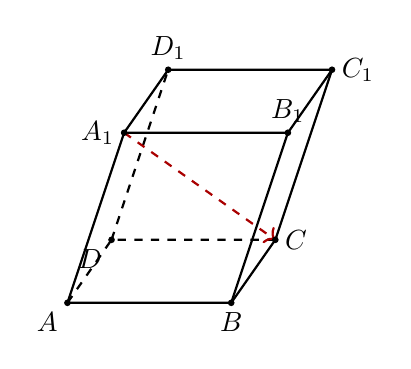
\begin{tikzpicture}[scale=0.8, baseline=(current bounding box.north)]
		\coordinate (A) at (0,0);
		\coordinate (B) at (2.6,0);
		\coordinate (C) at (3.3,1);
		\coordinate (D) at (0.7,1);
		\coordinate (A1) at (0.9,2.7);
		\coordinate (B1) at (3.5,2.7);
		\coordinate (C1) at (4.2,3.7);
		\coordinate (D1) at (1.6,3.7);
		\draw[thick] (A)--(B)--(C);
		\draw[thick, dashed] (A)--(D)--(C);
		\draw[thick] (A)--(A1);
		\draw[thick] (B)--(B1);
		\draw[thick] (C)--(C1);
		\draw[thick, dashed] (D)--(D1);
		\draw[thick] (A1)--(B1)--(C1)--(D1)--cycle;
		\draw[->, thick, dashed, DarkRed] (A1)--(C);
		\fill (A) circle (1.5pt) node[below left] {$A$};
		\fill (B) circle (1.5pt) node[below] {$B$};
		\fill (C) circle (1.5pt) node[right] {$C$};
		\fill (D) circle (1.5pt) node[below left] {$D$};
		\fill (A1) circle (1.5pt) node[left] {$A_1$};
		\fill (B1) circle (1.5pt) node[above] {$B_1$};
		\fill (C1) circle (1.5pt) node[right] {$C_1$};
		\fill (D1) circle (1.5pt) node[above] {$D_1$};
	\end{tikzpicture}
\end{minipage}

\category{10\quad $\bigstar\bigstar\bigstar$}

\begin{question}
	设向量$\overrightarrow{u}=(a,b,0)$，$\overrightarrow{v}=(c,d,1)$，其中$a^2+b^2=c^2+d^2=1$，则下列判断错误的是（\quad B\quad）
	
	\begin{tabular}{@{}l@{\quad}l@{}}
		A. 向量$\overrightarrow{v}$与$z$轴正方向夹角为定值 &
		B. $\overrightarrow{u}\cdot\overrightarrow{v}$的最大值为$\sqrt{2}$ \\[10pt]
		C. $\overrightarrow{u}$与$\overrightarrow{v}$的夹角最大值为$\dfrac{3\pi}{4}$ &
		D. $ad-bc$的最大值为$1$
	\end{tabular}
\end{question}
解：$|\overrightarrow{u}|=1$，$|\overrightarrow{v}|=\sqrt{2}$.
\begin{enumerate}[label=\Alph*.]
	\item $\cos\langle\overrightarrow{v},\overrightarrow{k}\rangle=\dfrac{1}{\sqrt{2}}=\dfrac{\sqrt{2}}{2}$，夹角恒为$45^\circ$，正确；
	\item $\overrightarrow{u}\cdot\overrightarrow{v}=ac+bd\le\sqrt{a^2+b^2}\cdot\sqrt{c^2+d^2}=1$，最大值为$1$，不是$\sqrt{2}$，\textbf{错误}；
	\item $\cos\langle\overrightarrow{u},\overrightarrow{v}\rangle=\dfrac{ac+bd}{\sqrt{2}}\in\left[-\dfrac{\sqrt{2}}{2},\dfrac{\sqrt{2}}{2}\right]$，夹角最大值为$\dfrac{3\pi}{4}$，正确；
	\item 设$a=\cos\alpha,\ b=\sin\alpha,\ c=\cos\beta,\ d=\sin\beta$，则$ad-bc=\sin(\beta-\alpha)\le1$，正确.
\end{enumerate}
故选 B.



\end{document}